% !TeX spellcheck = en_US
\subsection{Non-Equilibrium Work\label{Sec:FEM:NEW}}
\subsubsection{Non-Equilibrium Work for Free Energy Difference between Two States\label{Sec:FEM:NEW:StateFE}}
Non-Equilibrium Work (NEW) method for equilibrium free energy calculations was proposed by Jarzynski.\cite{JarzynskiPRL1997}. 
In 1997, Jarzynski showed
\begin{equation}
    \left< \exp\left[-\beta W(\tau)\right] \right> = \exp{(-\beta \Delta A)},
    \label{Eq:FEM:NEW:Jar}
\end{equation}
which is now called the Jarzynski equality. Here, $W$ is the accumulated work along a path $\lambda(t)$ connecting the initial and final states, with $\lambda(0)=0$ and $\lambda(\tau)=1$, and $\Delta A = A(1) - A(0)$ the free energy difference between these two states. 
$\left \langle \cdots \right \rangle$ in Eq.~\ref{Eq:FEM:NEW:Jar} is an average over a series of trajectories with the initial conditions chosen according to the equilibrium Boltzmann probability in state $\lambda(0)$. The path average samples all the realizations of dynamic paths weighted by their respective path actions under the time evolution of the system with an explicitly time-dependent Hamiltonian. This equality was also obtained by Crooks for Markovian and microscopically reversible dynamics.\cite{CrooksJSP1998} 

Now, we consider creating an equilibrium configuration for the state $\lambda=0$ and then slowly changing $\lambda$ from 0 to 1. As the coupling parameter advances, the system continues to sample phase space by molecular dynamics or Monte Carlo simulations, but under an explicitly time-dependent Hamiltonian. In the limit of a very slow transformation, the system will remain close to the equilibrium. The free energy difference can then be evaluated by changing $\lambda$ continuously
\begin{equation}
    \Delta A =\lim_{\tau\to\infty} \int_{0}^{\tau} {\frac{\partial{H\left[\textbf{x}(t);\lambda\right]}}{\partial{\lambda}}\bigg\rvert}_{\lambda=\lambda(t)} \dot{\lambda}(t) \diff t,
    \label{Eq:FEM:NEW:limitA}
\end{equation}  
where $\dot{\lambda}(t)$ is the time derivative of the coupling parameter $\lambda$. In Eq.~\ref{Eq:FEM:NEW:limitA}, the limit of $\tau\to\infty$ ensures that the transformation is performed infinitely slowly, and thus reversibly. The right-hand side of Eq.~\ref{Eq:FEM:NEW:limitA} is the ``reversible work'' done to the system during the transformation.

If the system is instead transformed between the initial and final states over a finite time interval $\tau$, the system will not be able to sample the phase space exhaustively at each value of $\lambda$, making this transformation irreversible. As the transformation proceeds, the system will be gradually driven out of equilibrium, causing hysteresis effects. From the second law of thermodynamic, it is expected that the work $W(\tau)$ performed during the nonequilibrium transformation is on average larger than or equal to the free energy difference between the two states
\begin{equation}
    \left \langle W(\tau) \right \rangle \ge \Delta A,
    \label{Eq:FEM:NEW:WA}
\end{equation} 
and the difference accounts for heat-dissipation effect. The work $W(\tau)$ performed on the system is the accumulated energy cost required to change the system
\begin{equation}
    W(\tau) = \int_{0}^{\tau} \frac{\partial{H[\textbf{x}(t);\lambda]}}{\partial{\lambda}}\bigg\rvert_{\lambda=\lambda(t)} \dot{\lambda}(t) \diff t
    \label{Eq:FEM:NEW:work}
\end{equation}    
The equality in Eq.~\ref{Eq:FEM:NEW:WA} will normally be achieved only if the transformation is infinitely slow, $\tau\to\infty$.  For paths of finite length, the amount of dissipated work, $\left \langle W(\tau) \right \rangle - \Delta A \ge 0$, depends on the chosen transformation path $\lambda(t)$.

Jarzynski equality, Eq.~\ref{Eq:FEM:NEW:Jar}, immediately leads to the second law in the form of Eq.~\ref{Eq:FEM:NEW:WA} because of the Jensen's inequality, $\left \langle e^{-x} \right \rangle \ge e^{-\left<x\right>} $.
Moreover, TI and TP can be thought as the limiting cases of the nonequilibrium process. When $\tau\to\infty$ or $\dot{\lambda}(t)\to0$, this is an infinitely slow transformation and the Eq.~\ref{Eq:FEM:NEW:limitA} is the formula of TI
\begin{equation}
    \Delta A = \int_{\lambda=0}^{\lambda=1}\left \langle \frac{\partial{H(\textbf{x},\textbf{p}_{x},\lambda)}}{\partial{\lambda}} \right \rangle_{\lambda} \diff\lambda
    \label{Eq:FEM:NEW:TINEW}
\end{equation}  
When $\tau\to0$ or $\dot{\lambda}(t)\to\infty$, this is an infinitely fast transformation where the configurations will not relax and the work is simply the change in the Hamiltonian when going from the initial to the final state,
\begin{equation}
    \lim_{\tau\to0}W(\tau) = H(\textbf{x}(0);\lambda=1)-H(\textbf{x}(0);\lambda=0)
    \label{Eq:FEM:NEW:limitW}
\end{equation}
Substituting the Eq.~\ref{Eq:FEM:NEW:limitW} into the Eq.~\ref{Eq:FEM:NEW:Jar}, the formula of TP can be recovered
\begin{equation}
    \Delta A = -\frac{1}{\beta} \ln \left \langle \exp[-\beta \Delta H(\textbf{x},\textbf{p}_{x})] \right \rangle _{0},
    \label{Eq:FEM:NEW:deltaA4NEW}
\end{equation}

\begin{figure}[htbp]
	\centering
	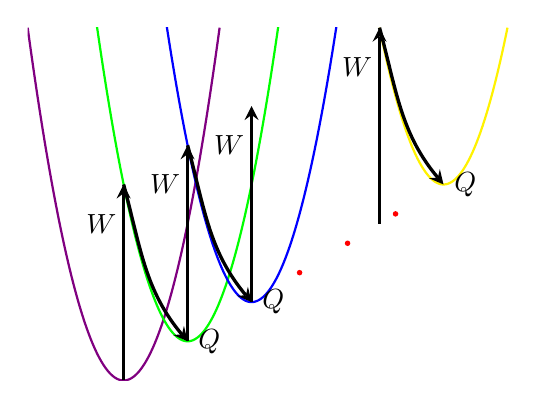
\begin{tikzpicture}
	\def\lims{xmin=-3,xmax=14,ymin=-0.001,ymax=9}
	\begin{axis}[\lims,hide x axis, hide y axis,width=0.7\textwidth,height=0.5\textwidth]
	\addplot[thick,violet,mark=none,samples=1000,domain=-3:3,y domain=-0.001:9] {0+(x-0)*(x-0)};
	\addplot[thick,green,mark=none,samples=1000,domain=-1:5,y domain=-0.001:9] {1+(x-2)*(x-2)};
	\addplot[thick,blue,mark=none,samples=1000,domain=1:7,y domain=-0.001:9] {2+(x-4)*(x-4)};
	\fill[red] (axis cs:5.5,2.75) circle[radius=1pt];
	\fill[red] (axis cs:7,3.5) circle[radius=1pt];
	\fill[red] (axis cs:8.5,4.25) circle[radius=1pt];
	\addplot[thick,yellow,mark=none,samples=1000,domain=8:12,y domain=-0.001:9] {5+(x-10)*(x-10)};
	\draw[very thick,->,>=stealth] (axis cs:0,0) to (axis cs:0,5);
	\draw[very thick,->,>=stealth] (axis cs:2,1) to (axis cs:2,6);
	\draw[very thick,->,>=stealth] (axis cs:4,2) to (axis cs:4,7);
	\draw[very thick,->,>=stealth] (axis cs:8,4) to (axis cs:8,9);
	\draw (axis cs:0-0.7,4) node{$W$};
	\draw (axis cs:2-0.7,5) node{$W$};
	\draw (axis cs:4-0.7,6) node{$W$};
	\draw (axis cs:8-0.7,8) node{$W$};
	\draw[very thick,->,>=stealth] (axis cs:0,5) to [out=285,in=130] (axis cs:2,1) node[right]{$Q$};
	\draw[very thick,->,>=stealth] (axis cs:2,6) to [out=285,in=130] (axis cs:4,2) node[right]{$Q$};
	\draw[very thick,->,>=stealth] (axis cs:8,9) to [out=285,in=130] (axis cs:10,5) node[right]{$Q$};
	
	\end{axis}
	
	\end{tikzpicture}
	\caption{The accumulation of work and heat along a nonequilibrium trajectory. The work is defined as the energy change when the coupling parameter switches from $\lambda_i$ to $\lambda_{i+1}$ with the coordinates fixed, while the dissipated heat is defined as the energy relaxation when the coordinate change with the coupling parameter fixed.}\label{Fig:FEM:NEW}
\end{figure}

%\begin{figure}[htbp]
%	\centering
%	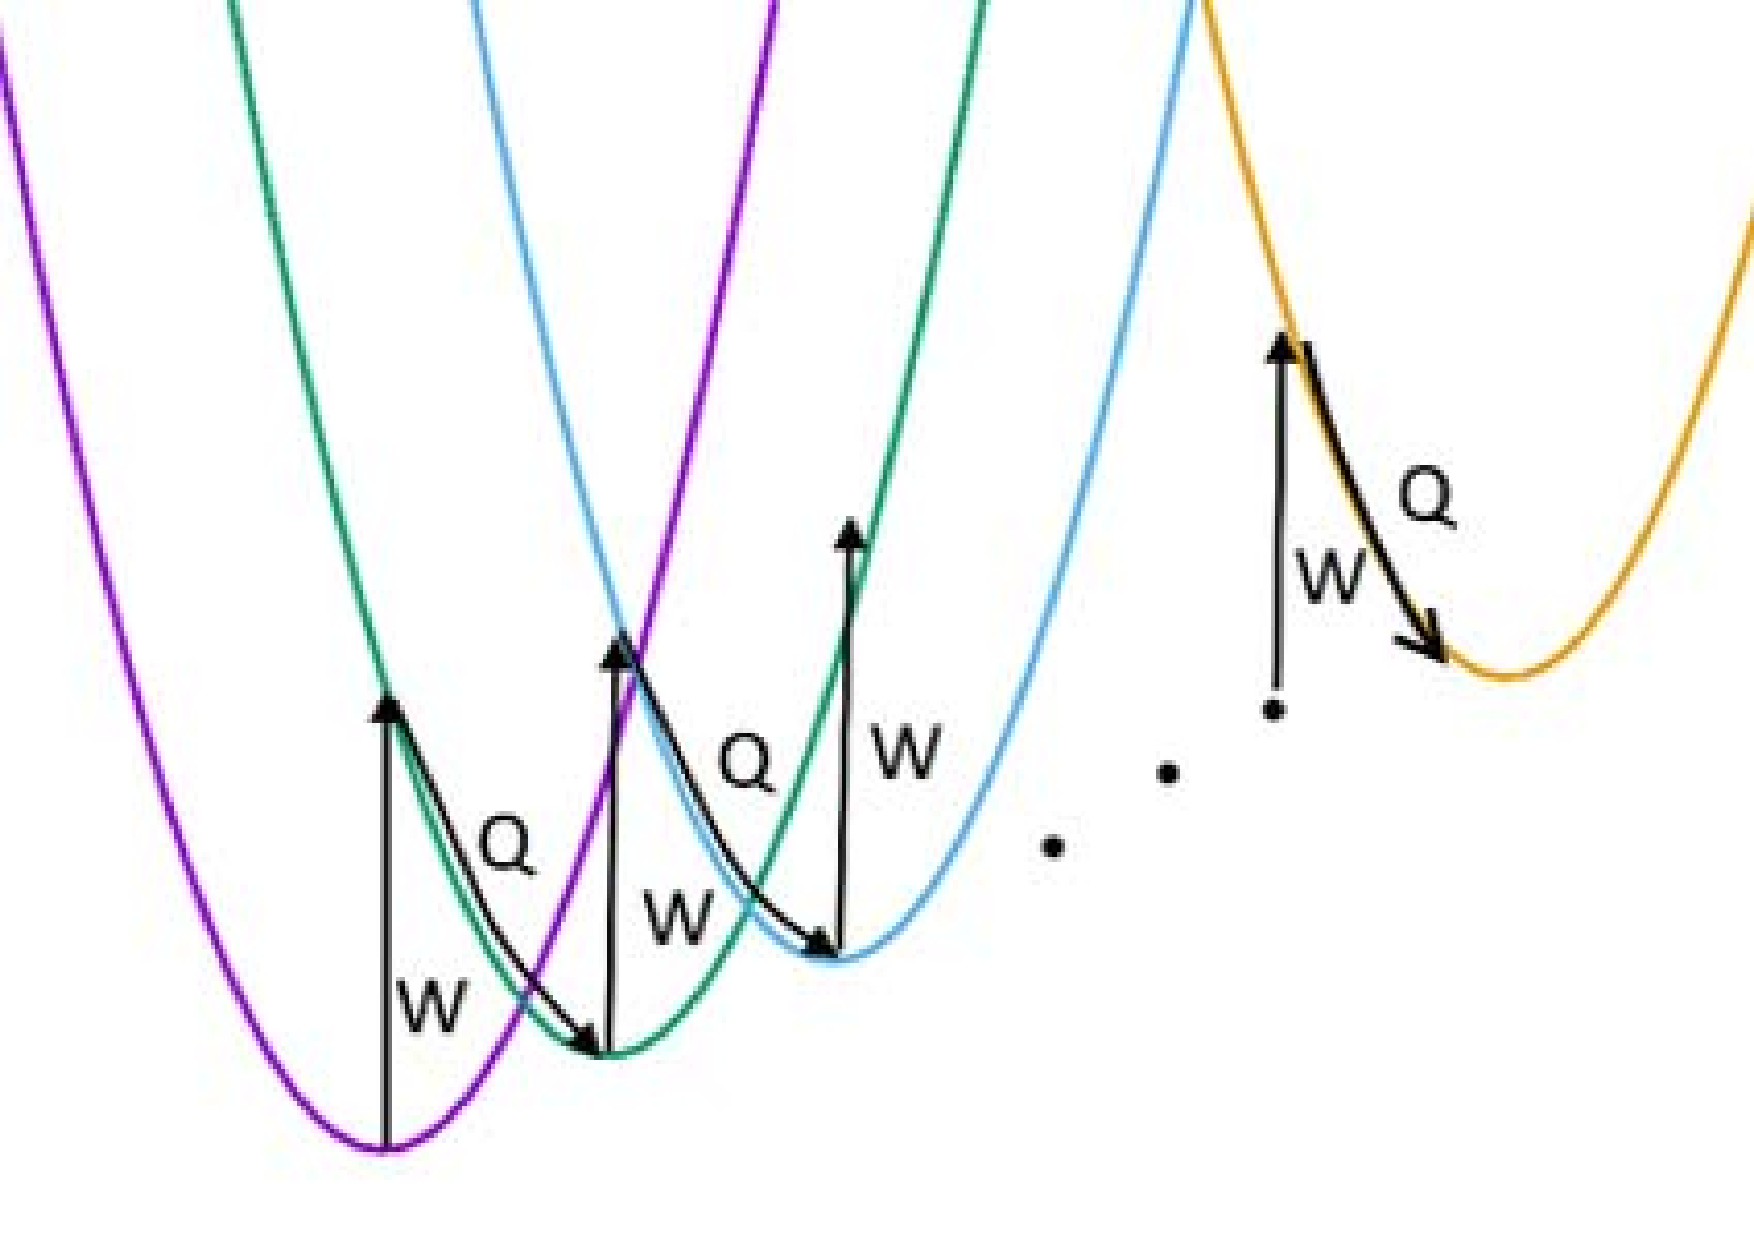
\includegraphics[width=0.4\textwidth]{figures/NEW.pdf}\\
%	\caption{The accumulation of work and heat along a nonequilibrium trajectory. The work is defined as the energy change when the coupling parameter switches from $\lambda_i$ to $\lambda_{i+1}$ with the coordinates fixed, while the dissipated heat is defined as the energy relaxation when the coordinate change with the coupling parameter fixed.}\label{Fig:FEM:NEW}
%\end{figure}

In Ref.~\cite{CrooksJSP1998}, Crooks showed that the distributions of work values from the forward and the backward paths satisfy a relation that is central to the histogram methods in free energy calculations
\begin{equation}
    \frac{p_{f}[w=W(\tau)]}{p_{b}[w=-\underline{W}(\tau)]}=\exp[\beta(w-\Delta A)],
    \label{Eq:FEM:NEW:crooks}
\end{equation}
where $p_{f}[w=W(\tau)]$ and $p_{b}[w=-\underline{W}(\tau)]$ are the probability densities of the work values in the forward and the reverse transformations (with a sign change for the work in the reverse path). Both are normalized, i.e., $\int p_{f}(w) \diff w=\int p_{b}(w) \diff w=1$. It is noted that Jarzynski equality Eq.~\ref{Eq:FEM:NEW:Jar} follows from Eq.~\ref{Eq:FEM:NEW:crooks} simply by integration over $w$ because the probability densities are normalized to 1:
\begin{equation}
    \int p_{f}(w)e^{-\beta w}\diff w=\int p_{b}(w)e^{-\beta \Delta A}\diff w,
    \label{Eq:FEM:NEW:crookstojar}
\end{equation}
Because of the normalization condition, the right-hand side is equal to $\exp(-\beta \Delta A)$, and Jarzynski equality follows. The bias, variance and mean square error of the Jarzynski estimator were studied by Gore et al.\cite{GorePNAS2003}

Following the Crooks Fluctuation Theorem (CFT),\cite{CrooksJSP1998} Bennett acceptance ratio can be applicable to nonequilibrium calculations. This approach was combined with a maximum likelihood estimate, and accurate free energy differences were obtained.\cite{ShirtsPRL2003}
In this approach, $\Delta A$ is calculated via
\begin{align}
    \sum_{i=1}^{n_{F}}\frac{1}{1+\exp \left[\beta(M+W_{i}-\Delta A)\right]} = \sum_{j=1}^{n_{R}}\frac{1}{1+\exp \left[-\beta(M+W_{j}-\Delta A)\right]},
    \label{Eq:FEM:NEW:NEBAR}
\end{align}
where $n_{F}$ and $n_{R}$ are the numbers of the forward and reverse transformations respectively, $W_{i}$ and $W_{j}$ are the work of forward and reverse measurements respectively, and $M=\beta^{-1}\ln(n_{F}/n_{R})$.
The corresponding statistical variance of $ \Delta A $, $ \sigma^2 $, is calculated using Eq.~10 in Ref.~\cite{ShirtsPRL2003}.

\subsubsection{Non-Equilibrium Work for Free Energy Profiles\label{Sec:FEM:NEW:FEP}}
When calculating the free energy profile in a pulling experiment, the Jarzynski equality is no longer straightforwardly applicable, because it relates the nonequilibrium work to free energy differences at different times, not positions along a predefined reaction coordinate. In order to surmount this difficulty, Hummer and Szabo extended the Jarzynski equality by measuring force/extension along pulling.\cite{HummerPNAS2001}

Let us begin with a system of which the phase-space density evolves according to a Liouville-type equation:
\begin{equation}
	\frac{\partial f(\mathbf{x},t)}{\partial t}=\mathscr{L}_tf(\mathbf{x},t).
	\label{Eq:FEM:NEW:Liouville}
\end{equation}
$\mathscr{L}_t$ is an explicitly time-dependent evolution operator that has the Boltzmann distribution as a stationary solution, $\mathscr{L}_t e^{-\beta \mathscr{H}(\mathbf{x},t)}=0$, where $\mathscr{H}(\mathbf{x},t)$ is a time-dependent Hamiltonian. For diffusive dynamics on a potential $V(\mathbf{x},t)$, the time evolution is governed by $\mathscr{L}_t=D\nabla e^{-\beta V(\mathbf{x},t)}\nabla e^{\beta V(\mathbf{x},t)}$, where $D$ is the diffusion coefficient and $\nabla=\partial/\partial \mathbf{x}$. Now consider the unnormalized Boltzmann distribution at time $t$,
\begin{align}
	p(\mathbf{x},t)=\frac{e^{-\beta \mathscr{H}(\mathbf{x},t)}}{\int e^{-\beta \mathscr{H}(\mathbf{x}^\prime,0)} \diff\mathbf{x}^\prime}.
\end{align}
Because this distribution is stationary ($\mathscr{L}_tp=0$), and because $\partial p/\partial t=-\beta(\partial \mathscr{H}/\partial t)p$, it follows that the above $p(\mathbf{x},t)$ is a solution of the sink equation
\begin{align}
	\frac{\partial p}{\partial t}=\mathscr{L}_tp-\beta\frac{\partial \mathscr{H}}{\partial t}p,
\end{align}
of which the solution, starting from an equilibrium distribution at time $t=0$, can be expressed as a path integral by using the Feynman-Kac theorem. Equating these two differential solutions immediately gives:
\begin{equation}
	\frac{e^{-\beta\mathscr{H}(\mathbf{x},t)}}{\int e^{-\beta \mathscr{H}(\mathbf{x}^\prime,0)} d\mathbf{x}^\prime}=\left\langle \delta(\mathbf{x}-\mathbf{x}_t)\exp{\left[-\beta\int_0^t\frac{\partial \mathscr{H}}{\partial t^\prime}(\mathbf{x}_{t^{\prime}},t^{\prime})\diff t^\prime\right]}\right\rangle.
	\label{Eq:FEM:NEW:SinkFK}
\end{equation}
The average $\left\langle \cdots \right\rangle$ is over an ensemble of trajectories starting from the equilibrium distribution at $t=0$ and evolving according to Eq.~\ref{Eq:FEM:NEW:Liouville}. Each trajectory is weighted with the Boltzmann factor of the external work $w_t$ done to the system,
\begin{equation}
	w_t=\int_0^t\frac{\partial \mathscr{H}}{\partial t^\prime}(\mathbf{x}_{t^{\prime}},t^{\prime})\diff t^\prime.
\end{equation}
Integrating on both sides of Eq.~\ref{Eq:FEM:NEW:SinkFK} with respect to $\mathbf{x}$, we obtain Jarzynski equality
\begin{equation}
	e^{-\beta \Delta G(t)}\equiv \frac{\int e^{-\beta\mathscr{H}(\mathbf{x},t)}\diff \mathbf{x}}{\int e^{-\beta \mathscr{H}(\mathbf{x},0)} d\mathbf{x}}=\left \langle e^{-\beta w_t}\right\rangle
\end{equation}
between the Boltzmann-averaged work $w_t$ and the equilibrium free energy difference $\Delta G(t)$ between times $t$ and $0$.

In a single-molecule pulling experiment, e.g. using atomic force microscope (AFM), the sample is moved at a constant speed $v$ relative to the cantilever with spring constant $k$. The position $z_t=vt+\delta z_t$ of the cantilever tip with respect to the sample is recorded, where $\delta z_t$ is the displacement of the cantilever tip. It can be described by a Hamiltonian $\mathscr{H}(\mathbf{x},t)=\mathscr{H}_0(\mathbf{x})+k(z(\mathbf{x})-vt)^2/2$, where $\mathscr{H}_0(\mathbf{x})$ is the Hamiltonian of the resting, unperturbed system. \textit{It is worth noting that $\mathscr{H}(\mathbf{x},t)$ is the Hamiltonian for the total system, including the cantilever.} Substituting this Hamiltonian into Eq.~\ref{Eq:FEM:NEW:SinkFK}, multiplying both sides by $\delta[z-z(\mathbf{x})]$, and integrating over all $\mathbf{x}$, we have
\begin{align}
	\frac{\int\delta[z-z(\mathbf{x})]e^{-\beta \left\{\mathscr{H}_0(\mathbf{x})+k[z(\mathbf{x})-vt]^2/2\right\}}\diff \mathbf{x}}{\int e^{-\beta \mathscr{H}(\mathbf{x},0)}\diff \mathbf{x}}=\qquad\qquad\qquad\qquad\qquad&\notag\\
	\int \delta[z-z(\mathbf{x})] \left\langle \delta(\mathbf{x}-\mathbf{x}_t)e^{-\beta\int_0^t -kv\left[z(\mathbf{x}_{t^\prime}-vt^\prime)\right] \diff t^\prime}\right\rangle \diff \mathbf{x}\notag\\
	\frac{\int\delta[z-z(\mathbf{x})]e^{-\beta \mathscr{H}_0(\mathbf{x})}\diff \mathbf{x}}{\int e^{-\beta \mathscr{H}(\mathbf{x},0)}\diff \mathbf{x}}e^{-\beta k(z-vt)^2/2}=\qquad\qquad\qquad\qquad\qquad\quad&\notag\\
	\left\langle \delta[z-z(\mathbf{x_{t}})] e^{-\beta \left[-kv\int_0^t z(\mathbf{x}_{t^\prime})\diff t^\prime+kv^2t^2/2\right]}\right\rangle\notag\\
	\frac{\int\delta[z-z(\mathbf{x})]e^{-\beta \mathscr{H}_0(\mathbf{x})}\diff \mathbf{x}}{\int e^{-\beta \mathscr{H}(\mathbf{x},0)}\diff \mathbf{x}}=\qquad\qquad\qquad\qquad\qquad\qquad\qquad\qquad&\notag\\
	\left\langle \delta[z-z(\mathbf{x_{t}})] e^{-\beta \left[kv^2t^2/2-kv\int_0^t z(\mathbf{x}_{t^\prime})\diff t^\prime-k(z(\mathbf{x}_t)-vt)^2/2\right]}\right\rangle
\end{align}
and finally taking the logarithm, we have:
\begin{align}
	G_0(z)\equiv&-\beta^{-1}\ln{\frac{\int\delta[z-z(\mathbf{x})]e^{-\beta \mathscr{H}_0(\mathbf{x})}\diff \mathbf{x}}{\int e^{-\beta \mathscr{H}_0(\mathbf{x})}\diff \mathbf{x}}}\notag\\
	      =&-\beta^{-1}\ln{\left<\delta(z-z_t)e^{-\beta \Delta w_t}\right>}-\beta^{-1}\ln{\frac{\int e^{-\beta \mathscr{H}_0(\mathbf{x})+k[z(\mathbf{x})]^2/2}\diff \mathbf{x}}{\int e^{-\beta \mathscr{H}_0(\mathbf{x})}\diff \mathbf{x}}}\notag\\
	      =&-\beta^{-1}\ln{\left<\delta(z-z_t)e^{-\beta \Delta w_t}\right>}+\delta G,
\end{align}
where $G_0(z)$ is the unperturbed free energy profile along the pulling coordinate $z$, and $\Delta w_t$ is the external work minus the instantaneous biasing potential, $\Delta w_t=w_t-k(z_t-vt)^2/2=kv(vt^2/2-\int_0^t z_{t^\prime}\diff t^\prime)-k(z_t-vt)^2/2$. %The expression can be obtained by integrating the power over time. At any moment $t^\prime$, the force acting on the system is $f=k(vt^\prime-z_{t^\prime})$. Correspondingly, the power $p=f\cdot v$. Therefore, $w_t=\int p\diff t^\prime=\int_0^t kv(vt^\prime-z_{t^\prime})\diff t^\prime=kv(vt^2/2-\int_0^t z_{t^\prime}\diff t^\prime)$. 
$\delta G$ is independent of time.
At time $t=0$, the trajectories are started from points $z_0$ drawn from a Boltzmann distribution corresponding to Hamiltonian $\mathscr{H}(\mathbf{x},0)=\mathscr{H}_0(\mathbf{x})+kz^2/2$, which is \emph{NOT} $\mathscr{H}_0(\mathbf{x})$.

At each time slice $t$, one can in principle obtain an estimate of the whole free energy surface. In practice with finite number of trajectories, at any given time $t$, only a narrow region around the equilibrium position $z=vt$ will be sampled adequately. Thus, an average over several time slices and repeated trajectories is required to obtain an optimal estimate of the free energy profile. At every time slice $t$, one obtains an ensemble of positions $z_t$ and corresponding $w_t$s. The position $z_t$ are binned, and the corresponding histogram values are incremented by $e^{-\beta w_t}$. The complete free energy profile $G_0(z)$ can be reconstructed by adapting the weighted histogram method:
\begin{align}
	G_0(z)=-\beta^{-1}\ln{\frac{\sum_t \frac{\left<\delta(z-z_t)\exp{(-\beta w_t)}\right>}{\left<\exp{(-\beta w_t)}\right>}}{\sum_t\frac{\exp{[-\beta u(z,t)]}}{\left<\exp{(-\beta w_t)}\right>}}},
	\label{Eq:FEM:NEW:FEprofile}
\end{align}
where the sum is over time slices $t$ and $u(z,t)=k(z-vt)^2/2$ is the time dependent biasing potential. As in the weighted histogram method, this procedure can be refined by making Eq.~\ref{Eq:FEM:NEW:FEprofile} self-consistent through replacement of $\left<\exp{(-\beta w_t)}\right>$ with
\begin{equation}
	\exp{[-\beta \Delta G(t)]}=\frac{\int \exp{\left\{-\beta \left[u(z,t)+G_0(z)\right]\right\}}\diff z}{\int \exp{\left\{-\beta[u(z,0)+G_0(z)]\right\}\diff z}},
\end{equation}
thus requiring an iterative solution for $\Delta G(t)$. Note that Eq.~\ref{Eq:FEM:NEW:FEprofile} can be rewritten as
\begin{equation}
	G_0(z)=-\beta^{-1}\ln{\frac{\sum_t \frac{\left<\delta(z-z_t)\exp{(-\beta \Delta w_t)}\right>\exp{[-\beta u(z,t)]}}{\left<\exp{(-\beta w_t)}\right>}}{\sum_t\frac{\exp{[-\beta u(z,t)]}}{\left<\exp{(-\beta w_t)}\right>}}},
\end{equation}
which is the natural logarithm of the weighted average of $\left<\delta(z-z_t)\exp{(-\beta \Delta w_t)}\right>$ over all the time slices with $\frac{\exp{[-\beta u(z,t)]}}{\left<\exp{(-\beta w_t)}\right>}$ being the weight.